\iffalse
	\chapter{2015}
	\author{AI24BTECH11003}
	\section{me}
\fi

%1
    \item In the assembly shown below, the part dimensions are: $L_1=22.0^{\pm0.01}mm$, $L_12=L_3=10.0^{\pm0.005}mm$. Assuming the normal distribution of part dimensions, the dimension $L_4$ in $mm$ for assembly condition would be:
    \hfill{(2015)}

    \begin{figure}[!ht]
\centering
\resizebox{0.3\textwidth}{!}{%
\begin{circuitikz}
\tikzstyle{every node}=[font=\normalsize]
\draw [ line width=1pt ] (8,16) rectangle (13.75,15);
\draw [ line width=1pt ] (8,15) rectangle (9,12.75);
\draw [ line width=1pt ] (12.75,15) rectangle (13.75,12.75);
\draw [ line width=1pt ] (9,13.75) rectangle (10.25,12.75);
\draw [ line width=0.9pt ] (10.25,13.75) rectangle (11.5,12.75);
\draw (9,12.75) to[short] (9,11.5);
\draw (10.25,12.75) to[short] (10.25,11.5);
\draw (11.5,12.75) to[short] (11.5,11.5);
\draw (12.75,12.75) to[short] (12.75,11.5);
\draw [<->, >=Stealth] (9,11.25) -- (12.75,11.25)node[pos=0.5, fill=white]{$L_1$};
\draw [<->, >=Stealth] (9,12.25) -- (10.25,12.25)node[pos=0.5, fill=white]{$L_2$};
\draw [<->, >=Stealth] (10.25,12.25) -- (11.5,12.25)node[pos=0.5, fill=white]{$L_3$};
\node [font=\normalsize] at (12,12.25) {$L_4$};
\end{circuitikz}
}%

\label{fig:my_label}
\end{figure}
    

    \begin{multicols}{4}
        \begin{enumerate}
            \item $2.0^{\pm0.008}$
            \item $2.0^{\pm0.012}$
            \item $2.0^{\pm0.016}$
            \item $2.0^{\pm0.020}$
        \end{enumerate}
    \end{multicols}

%2
    \item A DC welding power source has a linear voltage-current $\brak{V-I}$ characteristic with open circuit voltage of 300 A. For maximum arc power, the current (In Amperes) should be set as \rule{1cm}{0.15mm}
    \hfill{(2015)}

%3
    \item A triangular faucet in a CAD model has vertices $P_1\brak{0,0,0}$; $P_2\brak{1,1,0}$ and $P_3\brak{1,1,1}$. The area of the facet is
    \hfill{(2015)}

    \begin{multicols}{4}
        \begin{enumerate}
            \item $0.500$
            \item $0.707$
            \item $1.414$
            \item $1.732$
        \end{enumerate}
    \end{multicols}


%4
    \item Following data refers to the activities of a project where node 1 refers to the start and node 5 refers to the end of the project.

    \begin{table}[h]
        \centering
                \begin{tabular}{|c|c|} % c: center, |: vertical line
            \hline
            \textbf{Activity} & \textbf{Duration (days)} \\ % Header row
            \hline
            1-2   & 2 \\ % Row 1
            \hline
            2-3   & 1 \\ % Row 2
            \hline
            4-3   & 3 \\
            \hline
            1-4   & 3 \\
            \hline
            2-5   & 3 \\
            \hline
            3-5   & 2 \\
            \hline
            4-5   & 4 \\
            \hline
        \end{tabular}
        \label{tab:43}
    \end{table}

    The critical path (CP) in the network is
    \hfill{(2015)}
    
	\begin{multicols}{4}
		\begin{enumerate}
                \item $1-2-3-5$
                \item $1-4-3-5$
                \item $1-2-3-4-5$
                \item $1-4-5$
			\end{enumerate}
		\end{multicols}

%5
    \item For a canteen, the actual demand for disposable cups was 500 units in January and 600 units in February. The forecast for the month of January was 400 units. The forecast for the month of march considering smoothing coefficient as 0.75 is \rule{1cm}{0.15mm}
    \hfill{(2015)}

%6
    \item An orthogonal turning operation is carried out under the following conditions: rake angle$=5\degree$, spindle rotation speed $=400$rpm; axial feed $=0.4\frac{m}{min}$ and radial depth of cut $=5$mm. The chip thickness, $t_c$, is found to be 3mm. The shear angle (in degrees) in this turning process is \rule{1cm}{0.15mm}. 
    \hfill{(2015)}

%7

    \item The solidification time of a casting is proportional to $\brak{\frac{V}{A}}^2$, where $V$ is the volume of the casting, and $A$ is the total casting surface area losing heat. Two cubes of the same material and size are cast using sand casting process. The top face of one of the cubes is completely insulated. The ratio of the solidification time for the cube with top insulated to that of the other cube is
    \hfill{(2015)}

    \begin{multicols}{4}
        \begin{enumerate}
            \item $\frac{25}{36}$
            \item $\frac{36}{25}$
            \item $1$
            \item $\frac{6}{5}$
        \end{enumerate}
    \end{multicols}

%8
    
    \item In a slab rolling operation, the maximum thickness reduction $\brak{\Delta h_{max}}$ is given by $\Delta h_{max}=\mu^2R$, where $R$ is the radius of the roll and $\mu$ is the coefficient of friction between the roll and the sheet. If $\mu=0.1$, the maximum angle subtended by the deformation zone at the center of the roll (bite angle in degrees) is \rule{1cm}{0.15mm}
    \hfill{(2015)}

%9
        
    \item Considering massless rigid rod and small oscillations, the natural frequency (in $\frac{rad}{s}$) of vibration of the system shown in the figure is
    \hfill{(2015)}

    \begin{figure}[!ht]
\centering
\resizebox{0.35\textwidth}{!}{%
\begin{circuitikz}
    \draw[very thick] (-1,0) to[short, o-o] (0,0);
    \draw[very thick] (0,0) to [short, o-] (2,0);
    \draw[black] (2,0) to[short] ++(0,0.25) to[short, l={\footnotesize m=1kg}] ++(0.5,0) to[short] ++ (0,-0.5) to[short] ++(-0.5,0) to[short] ++(0,0.25);
    \draw[black] (0,0) to[short, o-] (0.125,-0.25);
    \draw[black] (0,0) to[short, o-] (-0.125,-0.25);
    \draw[black] (-0.15,-0.25) to[short] (0.15,-0.25);
    \draw[black] (-0.125, -0.25) to[short] (-0.145, -0.30);
    \draw[black] (-0.075, -0.25) to[short] (-0.095, -0.30);
    \draw[black] (-0.025, -0.25) to[short] (-0.045, -0.30);
    \draw[black] (+0.025, -0.25) to[short] (+0.005, -0.30);
    \draw[black] (+0.075, -0.25) to[short] (+0.055, -0.30);
    \draw[black] (+0.125, -0.25) to[short] (+0.105, -0.30);
    \draw[black] (-1,0) to [R, l_={\footnotesize $k=400\frac{N}{m}$},o-] (-1,2);
    \draw[black] (-1.15,2) to (-0.85,2);
    \draw[black] (-1.125, 2.05) to[short] (-1.145, 2.00);
    \draw[black] (-1.075, 2.05) to[short] (-1.095, 2.00);
    \draw[black] (-1.025, 2.05) to[short] (-1.045, 2.00);
    \draw[black] (-0.975, 2.05) to[short] (-0.995, 2.00);
    \draw[black] (-0.925, 2.05) to[short] (-0.945, 2.00);
    \draw[black] (-0.875, 2.05) to[short] (-0.895, 2.00);
    \draw[black] (0, -0.25) to[short] (0, -0.55);
    \draw [<->, >=Stealth] (-1,-0.5) -- (0,-0.5) node[pos=0.5, fill=white]{\footnotesize$r$};
    \draw [<->, >=Stealth] (2,-0.5) -- (0,-0.5) node[pos=0.5, fill=white]{\footnotesize$2r$};
    
\end{circuitikz}
}%

\label{fig:my_label}
\end{figure}

    \begin{multicols}{4}
        \begin{enumerate}
            \item $\sqrt{\frac{400}{1}}$
            \item $\sqrt{\frac{400}{2}}$
            \item $\sqrt{\frac{400}{3}}$
            \item $\sqrt{\frac{400}{4}}$
        \end{enumerate}
    \end{multicols}

%10
    
    \item For the truss shown in figure, the magnitude of force in member $PR$ and the support reaction at $R$ are respectively
    \hfill{(2015)}
    
    \begin{figure}[ht!]
\centering
\resizebox{0.221\textwidth}{!}{
    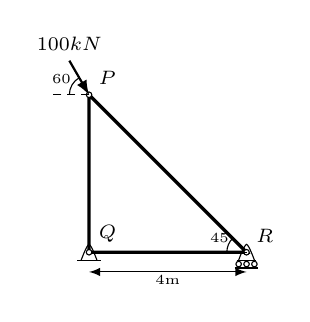
\begin{tikzpicture}
    \draw[black, very thick] (0,0) to (2,0) to (0,2) to (0,0);
    \filldraw[fill=white, draw=black] (0,0) circle (1pt) node[anchor=south west]{\scriptsize $Q$};
    \filldraw[fill=white, draw=black] (2,0) circle (1pt) node[anchor=south west]{\scriptsize $R$};
    \filldraw[fill=white, draw=black] (0,2) circle (1pt) node[anchor=south west]{\scriptsize $P$};
    \draw[black, thick, latex-] (0,2) to ++(-0.25,{sqrt(3)/4}) node[anchor=south]{\scriptsize$100kN$};
    \draw[black, densely dashed] (0,2) to ++(-0.5,0);
    \draw[thin] (-0.25, 2) arc[start angle=180, end angle=120, radius=0.25cm];
    \draw[thin] (1.75, 0) arc[start angle=180, end angle=135, radius=0.25cm];
    \draw[thin] plot [smooth] coordinates {(1.9, -0.1) (2, 0.1) (2.1, -0.1) };
    \draw[thin] (1.875,-0.1) to ++(+0.25,0);
    \draw[thin] (1.9, -0.15) circle (1pt);
    \draw[thin] (2.1, -0.15) circle (1pt);
    \draw[thin] (2.0, -0.15) circle (1pt);
    \draw[thin] (1.85,-0.2) to ++(+0.3,0);
    \draw[thin] plot [smooth] coordinates {(-0.1, -0.1) (0, 0.1) (0.1, -0.1)};
    \draw[thin] (-0.15,-0.1) to ++(+0.3,0);
    \draw[black] (2,0) to ++(-0.1,0) node[anchor=south east]{\tiny 45};
    \node at (-0.35, 2.2) {\tiny 60};
    \draw[black, latex-latex] (0,-0.25) to (2,-0.25);
    \node at (1,-0.35) {\tiny 4m};
\end{tikzpicture}
}
\end{figure}


    \begin{multicols}{2}
        \begin{enumerate}
            \item $122.47kN$ and $50kN$
            \item $70.71kN$ and $100kN$
            \item $70.71kN$ and $50kN$
            \item $81.65kN$ and $100kN$
        \end{enumerate}
    \end{multicols}

%11
    
    \item A ball of mass 0.1kg, initially at rest, is dropped from a height of 1m. Ball hits the ground and bounces off the ground. Upon impact with the ground, the velocity reduces by 20\%. The height (in m) to which the ball will rise is \rule{1cm}{0.15mm}
    \hfill{(2015)}

%12
    
    \item A pinion with radius $r_1$, and inertia $I_1$ is driving a gear with radius $r_2$ and inertia $I_2$. Torque $\tau_1$ is applied on pinion. The following are free body diagrams of pinion and gear showing important forces ($F_1$ and $F_2$) of interaction. Which of the following relations holds true?
    \hfill{(2015)}

    \begin{figure}[!ht]
\centering
\resizebox{0.75\textwidth}{!}{%
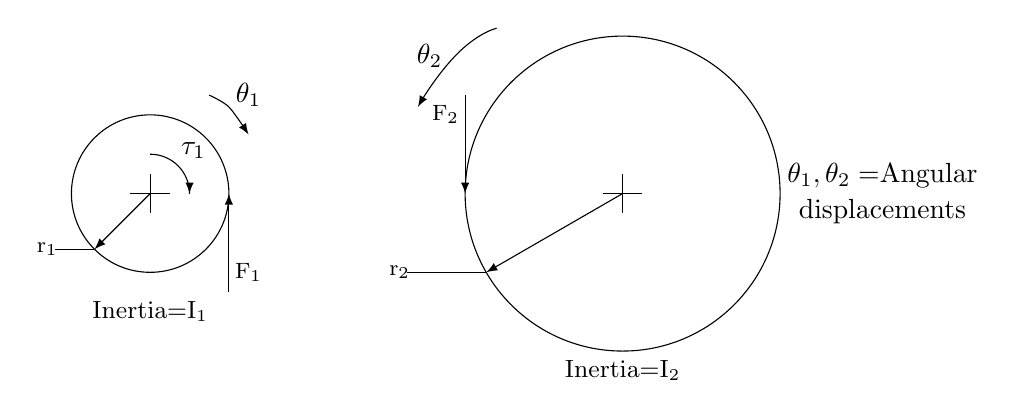
\begin{tikzpicture}
    \draw[black] (-2,0) circle (1);
    \node at (-2,-1.5){\small Inertia=I$_1$};
    \draw[black] (4,0) circle (2);
    \node at (4, -2.25){\small Inertia=I$_2$};
    \draw[black] (-2,0.25) to (-2,-0.25);
    \draw[black] (-1.75,0) to (-2.25,0);
    \draw[black] (4,0.25) to (4,-0.25);
    \draw[black] (3.75,0) to (4.25,0);
    \draw[black, latex-] (-1,0) to (-1,-1.25);
    \node at (-0.75,-1){\footnotesize F$_1$};
    \draw[black, latex-] (2,0) to (2,1.25);
    \node at (1.75,+1){\footnotesize F$_2$};
    \draw[black, -latex] (4,0) to ++(-{sqrt(3)}, -1);
    \draw[black] ({4-sqrt(3)},-1) to ++(-1,0);
    \node[black] at ({2.9-sqrt(3)},-1){\footnotesize r$_2$};
    \draw[black, -latex] (-2,0) to ++(-{sqrt(0.5)},-{sqrt(0.5)});
    \draw[black] ({-2-sqrt(0.5)}, -{sqrt(0.5)}) to ++(-0.5,0);
    \node[black] at ({-2.6-sqrt(0.5)},{-sqrt(0.5)}){\footnotesize r$_1$};
    \draw[black] (-2, 0.5) arc[start angle=90, end angle=0, radius=0.5];
    \node at (-1.45,0.55){$\tau_1$};
    \draw[black, latex-] (-1.5,0) to ++(0,0.001);
    \node at (7.3,0.23) {$\theta_1,\theta_2=$Angular};
    \node at (7.3,-0.23) {displacements};
    \draw[black, -latex] plot[smooth] coordinates {(-1.25,1.25) (-1.00,1.1) (-
    0.75,0.75)};
    \node at (-0.75,1.25) {$\theta_1$};
    \draw[black, -latex] plot[smooth, tension=1] coordinates {(2.4,2.1) (1.9,1.775) (1.4,1.1)};
    \node at (1.55,1.75){$\theta_2$};
\end{tikzpicture}
}%

\label{fig:my_label}
\end{figure}    

    \begin{enumerate}
        \item $F_1\neq F_2$;
        $\tau_1=I_1\Ddot{\theta} $;
        $ F_2=I_2\frac{r_1}{r_2^2}\Ddot{\theta}$
        \item $F_1= F_2;\tau_1=\left[I_1+I_2\brak{\frac{r_1}{r_2}}^2\right]\Ddot{\theta}; F_2=I_2\frac{r_1}{r_2^2}\Ddot{\theta}$
        \item $F_1= F_2;\tau_1=I_1\Ddot{\theta}; F_2=I_2\frac{1}{r_2}\Ddot{\theta}$
        \item $F_1\neq F_2;\tau_1=\left[I_1+I_2\brak{\frac{r_1}{r_2}}^2\right]\Ddot{\theta}; F_2=I_2\frac{1}{r_2}\Ddot{\theta}$
    \end{enumerate}


%13
    
    \item A mobile phone has a small motor with an eccentric mass used for vibrator mode. The location of the eccentric mass on motor with respect to center of gravity (CG) of the mobile and the rest of the dimensions of the mobile are shown. The mobile is kept on a flat horizontal surface. 

    \begin{figure}[!ht]
\centering
\resizebox{0.6\textwidth}{!}{%
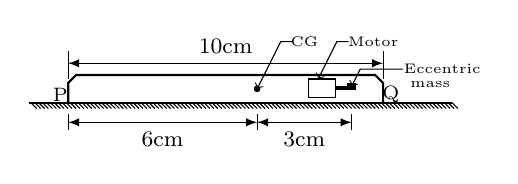
\begin{tikzpicture}
    \draw[black, thick] (-2.5,0) to (2.875,0);
    \draw[black, thick] (-2,0) to (-2,0.25) to (-1.9, 0.35) to (1.9,0.35) to (2.0,0.25) to (2.0,0);
    \foreach \x in {-2.475, -2.425, ..., 2.9} {
        \draw[black, thin] (\x, 0) -- (\x + 0.075, -0.075);
    }
    \draw[black, thin, latex-latex] (-2,0.5) -- (2,0.5) node[midway, above]{\footnotesize 10cm};
    \draw[black, thin] (-2,0.3) to (-2, 0.65);
    \draw[black, thin] (2,0.3) to (2, 0.65);
    \draw[black, thin, latex-latex] (-2, -0.25) -- (0.4,-0.25) node[midway, below]{\footnotesize 6cm};
    \draw[black, thin, latex-latex] (0.4, -0.25) -- (1.6,-0.25) node[midway, below]{\footnotesize 3cm};
    \draw[black, thin] (0.4, -0.35) to (0.4, -0.15);
    \draw[black, thin] (-2, -0.35) to (-2, -0.15);
    \draw[black, thin] (1.6, -0.35) to (1.6, -0.15);
    \filldraw[black] (0.4, 0.175) circle (1pt);
    \draw[black, thin, <-] (0.4, 0.175) to (0.7, 0.775) to (0.85, 0.775);
    \node at (1,0.775) {\tiny CG};
    \filldraw[black] (1.55,0.170) rectangle ++(0.1,0.075);
    \draw[black, very thick] (1.55, 0.185) to ++(-0.15,0);
    \draw[black] (1.4,0.185) to ++(0,0.115) to ++(-0.35,0) to ++(0,-0.24) to ++(0.35,0) to ++(0,0.125);
    \node at (-2.1,0.1){\scriptsize P};
    \node at (2.1,0.1){\scriptsize Q};
    \draw[black, thin, <-] (1.175, 0.3) to (1.4125,0.775) to (1.5625,0.775);
    \node at (1.875, 0.775) {\tiny Motor};
    \draw[black, thin, <-] (1.6,0.2075) to (1.70875,0.425) to (2.25,0.425);
    \node at (2.75,0.425){\tiny Eccentric};
    \node at (2.6, 0.225) {\tiny mass};
    
\end{tikzpicture}
}%

\label{fig:my_label}
\end{figure}

    Given in addition that the eccentric mass $=2$ grams, eccentricity $=2.19$ mm, mass of the mobile $=90$ grams, $g=9.81\frac{m}{s^2}$. Uniform speed of the motor in RPM for which the mobile will get just lifted off the ground at the end Q is approximately
    \hfill{(2015)}
    
    \begin{multicols}{4}
    \begin{enumerate}
        \item $3000$
        \item $3500$
        \item $4000$
        \item $4500$
    \end{enumerate}
    \end{multicols}		
